% !TeX root = ../../../graduate.tex
%% 第三章

\chapter{GEMM 专家知识获取与统一建模}
\chaptermark{GEMM 专家知识获取与统一建模}

第二章说明了高性能 GEMM 的调度决策同时受到寄存器分块、缓存分块、数据打包、向量化和边界处理等因素影响。Transform Dialect 可以显式表达 tiling、packing 和 vectorization 等变换，却不负责回答哪些候选能够调用给定微内核，也不判断某个库中的缓存参数能否迁移到当前编译与运行环境。BLIS 和 OpenBLAS 保存了经过工程实践固化的架构配置与内核实现，但这些信息服务于各自的 packing、调用约定和分派框架，并不直接构成调优器可消费的统一搜索空间\cite{VanZee2015BLIS,OpenMathLibOpenBLAS,LLVMProjectTransformDialect}。

直接复制高性能库中的 MR、NR、MC、KC 和 NC 等数值会混淆两类性质不同的知识。第一类是数据类型、指令集、寄存器块、packed layout 和调用约定等\emph{兼容性知识}，它决定候选能否通过特定后端正确执行；第二类是缓存块、候选顺序和向量化偏好等\emph{性能知识}，它只反映特定实现与平台上的经验，不应在缺少目标测量时被提升为全局硬约束。本文据此采用“后端专属硬 Contract 与可校准软先验分离”的建模原则：硬知识只来源于当前选定执行后端的真实接口，软知识保留来源、范围和置信度，并允许由在线反馈更新排序。

本章解决专家知识进入搜索空间之前的获取与统一建模问题。首先固定知识来源、执行后端和实验边界，并用真实 MLIR 编译测量说明通用参数空间存在的问题；随后给出半自动事实抽取与人工核验流程，将所得信息分别建模为 Expert Fact、Target Contract 和 Expert Rule；最后通过多来源冲突、第二数据类型 Contract、真实执行路径和贯穿案例验证三类对象的语义边界。本章输出的是第四章空间生成方法的结构化输入，不对最终最优调度作静态判定，也不把调优器本身作为本文贡献。

\section{问题上下文与知识来源边界}

本文将知识来源、目标执行后端和实际测量主机分别记录。主要知识源为 BLIS 提交 \texttt{36df51a81cc732eeadbf2e6732941dd5400db47d}，补充知识源为 OpenBLAS 提交 \texttt{b338322e9afc063d95e2c117e85bedf28213295a}。BLIS Haswell 配置提供 \texttt{f32} $6\times16$ 与 \texttt{f64} $6\times8$ 微内核、缓存分块和 pack kernel 事实；OpenBLAS 提供 Haswell 与 RISC-V 目标的独立内核形状和 blocking 配置。两者即使面向相同 ISA 和数据类型，也具有不同的 packing 语义与调用 ABI，因此不能把两个库的寄存器块事实合并为同一个硬 Contract。

当前 x86 执行后端选择 BLIS Haswell 微内核。主数据类型为 \texttt{f32}，用于贯穿案例和完整路径验证；\texttt{f64} 用于检验同一 Schema、packing pass 和调用适配器能否表达第二个真实 Contract。知识源架构为 Intel Haswell，所需指令特性为 AVX2 与 FMA。实际测量主机为 Intel Core i7-10750H，属于 Comet Lake。该主机与知识源不是同一微架构，但提供实验所需的 ISA 特性。因此，本章结果只支持 ISA 兼容条件下的本机验证，不能解释为 Haswell 原生性能，也不能证明跨主机排序稳定。

LLVM/MLIR 固定在提交 \texttt{09b849a2ac83dbf4be1b2f01c767339e46cc34ae}，Buddy 工作区固定在提交 \texttt{d7bb40cbac731175dc507f06f0655d81508f2ca2}。RISC-V 侧已经抽取 BLIS 与 OpenBLAS 的 RVV 配置，并生成 K230 可部署 ELF；由于尚无板端返回结果，RISC-V 事实只能用于展示来源隔离和 Contract 表达能力，不能进入本章的性能结论。第二台 x86 主机同样处于待运行状态。

对知识源 $s$，本文把可抽取知识划分为

\begin{equation}
\mathcal{K}^{(s)}
=
\mathcal{K}_{\mathrm{compat}}^{(s)}
\cup
\mathcal{K}_{\mathrm{perf}}^{(s)},
\label{eq:chapter3-knowledge-classes}
\end{equation}

其中 $\mathcal{K}_{\mathrm{compat}}^{(s)}$ 包括 dtype、ISA、MR/NR、packed layout、stride、tail 和 call ABI；$\mathcal{K}_{\mathrm{perf}}^{(s)}$ 包括 MC/KC/NC 或 P/Q/R、候选顺序、向量化偏好及其条件。只有当来源 $s$ 与实际选择的 Target Contract 一致时，兼容性事实才能形成该后端的硬约束。性能事实无论来自何种库，在完成目标校准前均保持为软先验。

知识获取过程中还需区分四类字段。第一类可由源码直接抽取，例如微内核符号、MR、NR、MC、KC、NC、pack kernel 和编译 ISA 标志；第二类需要确定性推导或人工判断，例如由向量位宽与元素位宽推导 lane 数，以及对不完整 packed layout 的语义标注；第三类属于 Target Contract，用于描述内核固有要求、适配器可补偿条件和 fallback；第四类来自实验，包括编译状态、数值正确性、预测路径、实际路径、符号替换和运行时间。四类字段分别保留来源与状态，防止把源码事实、接口模型和实测结果混写为同一种“专家经验”。

\section{通用调度空间的预备实证分析}

本节只回答“通用空间中是否存在足以支持后续研究的问题”，不承担第六章的完整性能比较。预备实验选取 8 个 \texttt{f32} 静态 shape，包括 $64^3$、$96^3$、$128^3$、$192^3$ 四个方形矩阵，以及 $64\times32\times256$、$128\times256\times64$、$32\times256\times256$ 和 $192\times256\times256$ 四个非方形矩阵。本文统一按照 $M\times K\times N$ 记录 shape。

通用空间由三个独立 tile 参数和一个向量化开关构成：

\begin{equation}
\begin{aligned}
T_M &\in \{4,6,8,12,16,24,32\},\\
T_N &\in \{4,8,12,16,24,32\},\\
T_K &\in \{8,16,32,64\},\\
V   &\in \{0,1\}.
\end{aligned}
\label{eq:chapter3-generic-domain}
\end{equation}

每个 shape 的原始空间规模为 $7\times6\times4\times2=336$。预备检查只包含两条最小合法性条件：tile 不超过对应静态维度；启用 \texttt{f32} AVX2 向量化时，$T_N$ 为 8 个 lane 的整数倍。该检查并不包含 packing、call ABI 和 tail adapter，不能等同于第四章的完整 Compatibility Checker。经过检查，7 个 shape 的合法空间为 280，缩减 16.7\%；$K=32$ 的 $64\times32\times256$ shape 合法空间为 210，缩减 37.5\%。

实验使用随机种子 17，在每个 shape 的合法空间中采样 6 个候选，并从拒绝集合保留 2 个代表点；每个 shape 另运行 1 个未分块基线。原始日志包含 72 行，其中 48 个候选进入真实 Transform/LLVM/Clang 流程，16 个候选在策略检查阶段被拒绝，8 行为未分块基线。执行链为

\begin{equation}
\texttt{linalg.matmul}
\rightarrow \text{Transform 实例化}
\rightarrow \text{LLVM IR}
\rightarrow \text{Clang AOT}
\rightarrow \text{执行与数值校验}.
\label{eq:chapter3-preliminary-pipeline}
\end{equation}

每个候选预热 1 次，测量 3 次，每次包含 3 次内层迭代。数值比较满足

\begin{equation}
\left|c_{ij}-\hat{c}_{ij}\right|
\leq 10^{-3}+10^{-4}\left|\hat{c}_{ij}\right|,
\label{eq:chapter3-correctness-tolerance}
\end{equation}

其中 $c_{ij}$ 为候选输出，$\hat{c}_{ij}$ 为参考结果。为比较不同 shape 内部的候选质量，本文定义

\begin{equation}
\widetilde{P}_{s,i}
=
\frac{P_{s,i}}{\max_{j\in\mathcal{M}_s}P_{s,j}},
\qquad
B_s(b)=\max_{1\leq i\leq b}\widetilde{P}_{s,i},
\label{eq:chapter3-preliminary-metrics}
\end{equation}

其中 $\mathcal{M}_s$ 为 shape $s$ 的 6 个实测候选，$B_s(b)$ 表示预算 $b$ 下的 best-so-far。

\begin{figure}[!htbp]
  \centering
  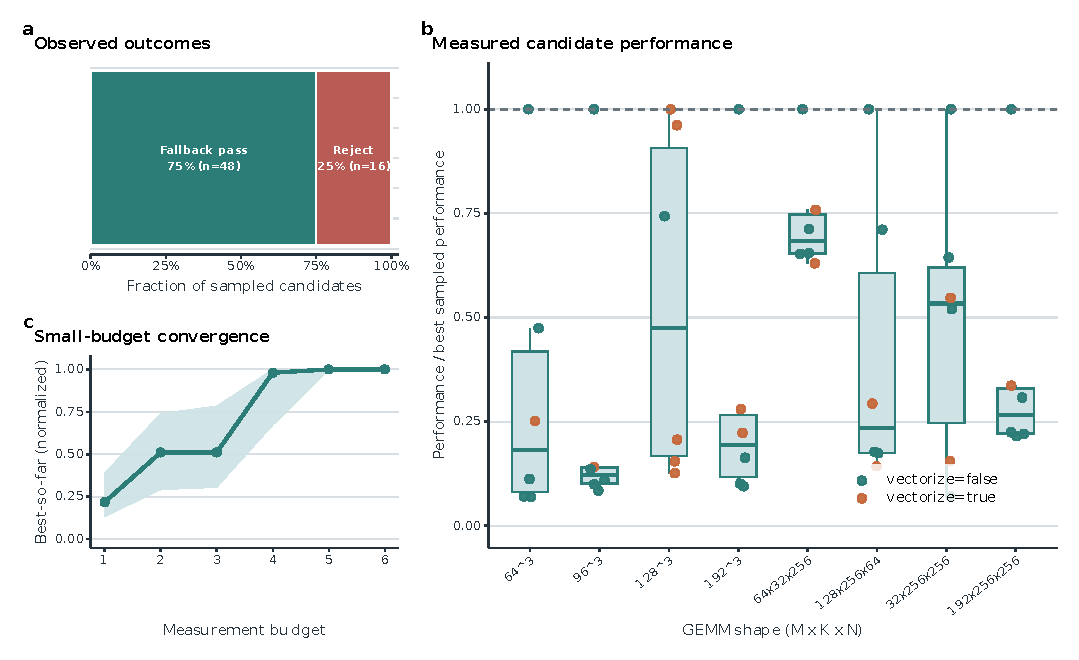
\includegraphics[width=\textwidth]{../experiments/chapter3_rules/figures/fig3-1_preliminary_distribution.pdf}
  \caption{通用 Transform 调度空间的预备实验结果。a，8 个 \texttt{f32} shape 上 64 个候选的观测结果构成；b，每个 shape 的 6 个已测候选相对该 shape 最优样本的归一化性能，颜色区分是否启用 Transform 向量化；c，6 次测量预算下 8 个 shape 的 best-so-far 中位数与四分位区间。随机种子为 17。}
  \label{fig:chapter3-preliminary-distribution}
\end{figure}

如图~\ref{fig:chapter3-preliminary-distribution} 所示，16 个静态拒绝占候选统计的 25\%，48 个实际尝试候选均完成 Transform、LLVM lowering、本地编译、执行和正确性检查，占 75\%。实际尝试候选的编译成功率和正确率均为 100\%。由于该冻结预备模板当时只实现 tiling 与可选 vectorization，没有物化 BLIS packed panel，也没有生成 BLIS 调用，48 个正确候选全部观测为 fallback，microkernel replacement 为 0\%。

48 个候选的归一化性能中位数为 0.265，范围为 0.070--1.000；相对各 shape 未分块默认路径的加速比中位数为 1.683，单候选本地编译时间中位数为 2955.9 ms。该结果说明：通用空间存在可在编译前识别的不兼容组合；通过最小合法性检查的候选仍具有分散的性能分布；Contract 预测本身不会自动产生真实微内核调用。后续 packing 与调用适配器已经补齐，但本节保留原始 fallback 记录，不用后续结果改写预备实验历史。

\section{专家事实抽取方法}

BLIS 将架构相关配置集中在 context 初始化函数中，并通过注册表关联数据类型、块尺寸、pack kernel 和 GEMM microkernel，为结构化抽取提供了明确入口\cite{VanZee2015BLIS}。本文的 BLIS Fact Extractor 以 \texttt{config/haswell/bli\_cntx\_init\_haswell.c} 为主入口，同时读取 \texttt{config/haswell/make\_defs.mk} 和对应 kernel 实现。OpenBLAS 抽取器则沿目标配置、GEMM kernel、blocking 宏和构建目标追踪事实。两条路径均采用“自动解析、机器交叉检查、人工签核队列”的半自动方法，不声称理解任意 C 预处理表达式或手写汇编的全部语义。

抽取过程包含五个步骤。

\textbf{（1）版本与激活分支冻结。} 提取器记录库提交，定位目标架构的激活配置，并解释当前需要的字面量 \texttt{\#if 0}、\texttt{\#if 1}、\texttt{\#else} 和 \texttt{\#endif}。复杂条件编译与运行时分派若无法由当前解析器闭合，则进入人工核验队列。

\textbf{（2）字段解析。} BLIS 路径匹配 \texttt{GEMM\_UKR}、\texttt{PACKM\_KER}、\texttt{bli\_blksz\_init\_easy} 和构建标志，恢复 kernel、MR/NR、MC/KC/NC、pack kernel 与 ISA。OpenBLAS 路径恢复目标、kernel 形状及 P/Q/R 等 blocking 参数，并保留原库字段名。

\textbf{（3）跨位置交叉检查。} BLIS 提取器根据 kernel 符号定位实现文件，读取对应 kernel setup 宏声明的 MR/NR，并与 context 数值比较。单精度路径的 MR=6、NR=16 与双精度路径的 MR=6、NR=8 均得到独立印证。OpenBLAS 通过固定版本构建和 4 个 shape、28 条正确运行记录验证公开 SGEMM 前端可执行，但该验证不被解释为两个库的内部 microkernel ABI 可以互换。

\textbf{（4）原子化与归一化。} 一个配置 profile 被拆分为字段级 Fact。kernel 符号、寄存器块、缓存块、pack kernel、ISA 和向量 lane 分别拥有独立标识、来源位置和证据状态。这样，规则只引用真正参与决策的事实，单个字段变化时也可局部复核。

\textbf{（5）核验、冲突与歧义输出。} 提取器同时生成 Schema 校验结果、人工核验项、冲突记录和开放歧义。BLIS Haswell 主成果包含 22 条原子 Fact，必需字段覆盖率、源码可追溯率和机器检查通过率均为 100\%；16 条人工核验记录均由论文作者签核为 \texttt{verified}。多来源扩展形成 BLIS Haswell、BLIS RVV、OpenBLAS Haswell 和 OpenBLAS RISC-V 四个来源--目标 profile，并记录 4 个跨来源冲突。

\section{专家事实统一表示}

Expert Fact 的职责是保存“在固定来源和作用范围内观察到什么”，而不是直接决定候选接受、排序或拒绝。本文将 Fact 表示为

\begin{equation}
f
=
\langle id,\;scope,\;source,\;value,\;evidence,\;state\rangle,
\label{eq:chapter3-fact-model}
\end{equation}

其中 $scope$ 描述算子、数据类型、架构、指令特性和线程模式；$source$ 保存库、版本、文件、行号和符号；$value$ 同时保存原始表达与归一化值；$evidence$ 表示证据等级和抽取方式；$state$ 分别记录机器检查与人工核验。表~\ref{tab:chapter3-fact-schema} 给出主要字段。

\begingroup
\small
\begin{longtable}{@{}p{0.22\textwidth}p{0.16\textwidth}p{0.54\textwidth}@{}}
  \caption{Expert Fact Schema 字段定义}\label{tab:chapter3-fact-schema}\\
  \toprule
  \textbf{字段} & \textbf{类型} & \textbf{定义} \\
  \midrule
  \endfirsthead
  \toprule
  \textbf{字段} & \textbf{类型} & \textbf{定义} \\
  \midrule
  \endhead
  \texttt{fact\_id} & 必需 & 全局唯一的字段级事实标识，用于规则引用和 provenance 连接。 \\
  \texttt{operator} & 必需 & 源算子的语义类别，本章为 GEMM，并映射到 \texttt{linalg.matmul}。 \\
  \texttt{dtype} & 必需 & 元素数据类型，本章主 Contract 覆盖 \texttt{f32} 与 \texttt{f64}。 \\
  \texttt{architecture} & 必需 & 知识源的目标架构与 ISA 范围。 \\
  \texttt{library} & 必需 & 事实来源库及来源 profile，禁止跨库静默合并。 \\
  \texttt{version} & 必需 & 不可变的源码提交标识。 \\
  \texttt{source\_file} & 必需 & 相对来源库根目录的源码路径。 \\
  \texttt{source\_line} & 必需 & 一基源码行号。 \\
  \texttt{source\_symbol} & 必需 & 包含该事实的函数、宏或配置符号。 \\
  \texttt{raw\_value} & 必需 & 自动抽取或确定性解码得到的原始值。 \\
  \texttt{normalized\_field} & 必需 & 统一语义字段名，如 \texttt{mr}、\texttt{nr} 或 \texttt{isa}。 \\
  \texttt{normalized\_value} & 必需 & 通过 Schema 校验的归一化类型和值。 \\
  \texttt{applicability} & 必需 & 算子、目标、数据类型、指令特性和线程模式等适用范围。 \\
  \texttt{evidence\_level} & 必需 & E1--E5 证据等级。 \\
  \texttt{extraction\_mode} & 必需 & 自动抽取、确定性推导、人工标注或实验校准。 \\
  \texttt{verification\_status} & 必需 & 机器检查与人工签核状态，二者不得互相替代。 \\
  \texttt{notes} & 必需 & 推导说明、歧义、限制与复核提示。 \\
  \bottomrule
\end{longtable}
\endgroup

BLIS Haswell 的 22 条 Fact 由两种数据类型各 11 个字段组成。单精度事实包括 MR=6、NR=16、MC=168、KC=256、NC=4080、256 bit 向量和 8 个 \texttt{f32} lane；双精度事实包括 MR=6、NR=8、MC=72、KC=256、NC=4080、256 bit 向量和 4 个 \texttt{f64} lane。MR/NR 由于得到 kernel setup 宏的独立印证而标记为 E2；向量 lane 由 ISA 位宽与元素宽度确定性推导，标记为 E3。MC/KC/NC 虽然是 E1 源码事实，但仍属于该来源 profile 的性能配置，不能仅凭证据等级转化为跨主机硬约束。

\section{目标微内核 Contract 建模}

Fact 说明源码中存在某个值，Target Contract 则回答实际执行后端在什么条件下可以被正确调用。例如，MR=6、NR=16 是源码事实；候选能否调用对应微内核，还需同时检查 dtype、ISA、A/B packed layout、步长、K 维行为、M/N tail 和 call ABI。本文将 Contract 表示为

\begin{equation}
\mu
=
\langle kernel,\;scope,\;requirements,\;adapter,\;fallback,\;evidence\rangle,
\label{eq:chapter3-contract-model}
\end{equation}

其中 $requirements$ 是微内核不可妥协的接口条件，$adapter$ 是后端已实现且可验证的有限补偿，$fallback$ 是专用内核不可用时的正确通用路径。Contract 对 direct 的预测不等于已经发生 replacement；实际路径还取决于 packing pass、调用适配器、链接符号和运行时 tail 分支。

\begingroup
\small
\begin{longtable}{@{}p{0.24\textwidth}p{0.15\textwidth}p{0.53\textwidth}@{}}
  \caption{Target Contract Schema 字段定义}\label{tab:chapter3-contract-schema}\\
  \toprule
  \textbf{字段} & \textbf{类型} & \textbf{定义} \\
  \midrule
  \endfirsthead
  \toprule
  \textbf{字段} & \textbf{类型} & \textbf{定义} \\
  \midrule
  \endhead
  \texttt{kernel\_id} & 必需 & 目标微内核 Contract 的唯一标识。 \\
  \texttt{backend\_id} & 必需 & 实际可调用后端及其来源 profile。 \\
  \texttt{dtype} & 必需 & 内核支持的元素数据类型。 \\
  \texttt{isa} & 必需 & 调用内核所需的指令集特性。 \\
  \texttt{mr/nr} & 必需 & 固定输出寄存器块尺寸。 \\
  \texttt{k\_constraint} & 必需 & K 的最小值、主循环步长和 remainder 行为。 \\
  \texttt{input\_layout} & 必需 & A/B 在内核边界处的 packed panel 语义。 \\
  \texttt{output\_layout} & 必需 & 输出存储偏好与写回语义。 \\
  \texttt{stride} & 必需 & packed panel 与 C 输出步长约束。 \\
  \texttt{alignment} & 必需 & 已知字节对齐或显式未知状态。 \\
  \texttt{packing} & 必需 & direct 路径的 packing 要求与 pack kernel。 \\
  \texttt{tail\_policy} & 必需 & 内核自身行为及 adapter 的 M/N/K 补偿方式。 \\
  \texttt{call\_convention} & 必需 & 可调用 ABI 与参数语义。 \\
  \texttt{fallback\_path} & 必需 & direct/adapt 不可用时的正确执行路径。 \\
  \texttt{adapter\_capabilities} & 必需 & packing、padding、fringe 和 remainder 等已实现能力。 \\
  \texttt{verification\_status} & 必需 & 源码交叉检查、运行时路径与正确性状态。 \\
  \bottomrule
\end{longtable}
\endgroup

当前 x86 后端建立两个真实 Contract。\path{haswell_f32_gemm_6x16} 对应 \path{bli_sgemm_haswell_asm_6x16}，要求 AVX2/FMA、MR=6、NR=16 和 packed A/B panel；\path{haswell_f64_gemm_6x8} 对应 \path{bli_dgemm_haswell_asm_6x8}，要求 MR=6、NR=8 和对应双精度 packed panel。两个 Contract 均把通用 MLIR 路径作为 fallback。OpenBLAS Haswell 的 $8\times4$ 和 BLIS Haswell 的 $6\times16$ 分别形成后端专属 Contract，不因 ISA 相同而合并。

给定候选 $p$ 和 Contract $\mu$，兼容性由字段谓词共同决定：

\begin{equation}
\begin{aligned}
\mathrm{Compat}(p,\mu)
=\;&
\phi_{\mathrm{dtype}}
\land\phi_{\mathrm{isa}}
\land\phi_{\mathrm{mr,nr}}
\land\phi_{k}\\
&\land\phi_{\mathrm{layout}}
\land\phi_{\mathrm{stride}}
\land\phi_{\mathrm{align}}
\land\phi_{\mathrm{packing}}
\land\phi_{\mathrm{tail}}
\land\phi_{\mathrm{call}}.
\end{aligned}
\label{eq:chapter3-contract-compatibility}
\end{equation}

若全部要求均满足，候选进入 direct；若不满足项属于已实现且可验证的有限补偿，候选进入 adapt；若专用内核不可用但存在正确通用 lowering，候选进入 fallback；违反语义、Transform 合法性或不存在正确退化路径的候选进入 reject。

后续正式语料验证了该分类不是纸面接口。单精度语料包含 1256 个候选--shape 实测案例，其中 direct、adapt 和 fallback 分别为 416、440 和 400，预测与运行时观测一致率为 100\%。双精度扩展覆盖 36 个 shape 和 3024 条候选观测，其中 direct 为 756，adapt 为 2268，预测路径与 runtime fringe 观测同样全部一致。这里的 100\% 只表示当前行主序、单线程、已实现 Contract 范围内的一致性，不代表任意 stride、更多 ISA 或跨主机上的普遍准确率。

\section{专家规则构建方法}

Expert Rule 将 Fact 和 Contract 转化为候选生成、过滤或排序动作。本文将规则表示为

\begin{equation}
\begin{aligned}
r=\langle&
id,\;condition,\;action,\;domain,\;strength,\;priority,\\
&source,\;scope,\;evidence,\;conflict,\;provenance
\rangle .
\end{aligned}
\label{eq:chapter3-rule-model}
\end{equation}

$condition$ 描述触发条件，$action$ 描述生成、约束、排序、适配或退化动作，$domain$ 给出条件参数域，$strength$ 区分硬约束、条件硬约束和软先验，$priority$ 与 $conflict$ 用于显式处理冲突。规则构建遵循“先接口、后性能”的顺序：首先由 Target Contract 形成 dtype、ISA、MR/NR、packing 与 fallback 约束；随后将 cache blocking、向量 lane 和 shape 关系转化为候选域或排序特征；最后为未满足专用路径的候选生成 adapt、fallback 或 reject。

\begin{figure}[!htbp]
  \centering
  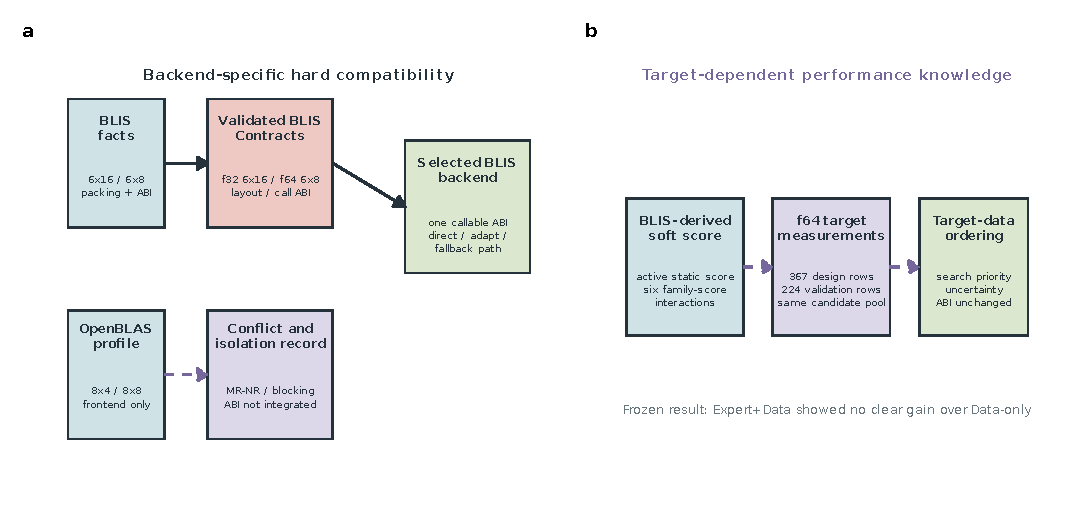
\includegraphics[width=\textwidth]{../experiments/chapter3_rules/figures/fig3-2_fact_contract_rule_boundary.pdf}
  \caption{兼容性知识与性能知识的建模边界。a，BLIS 与 OpenBLAS 的寄存器块、packing 和调用约定分别进入后端专属 Contract，运行时只选择一个实际可调用 ABI；b，cache blocking 等性能知识以来源标记的软先验进入目标校准，只改变初始点和候选顺序，不改变正确性约束。}
  \label{fig:chapter3-object-boundary}
\end{figure}

表~\ref{tab:chapter3-rule-schema-examples} 给出五类已实现规则。每一行均对应成果包中的真实 YAML 对象。

\begingroup
\small
\begin{longtable}{@{}p{0.21\textwidth}@{\hspace{1.2em}}p{0.48\textwidth}@{\hspace{1.2em}}p{0.21\textwidth}@{}}
  \caption{Rule Schema 与真实规则示例}\label{tab:chapter3-rule-schema-examples}\\
  \toprule
  \textbf{规则标识/类别} & \textbf{条件、动作与参数域} & \textbf{强度/优先级/证据} \\
  \midrule
  \endfirsthead
  \toprule
  \textbf{规则标识/类别} & \textbf{条件、动作与参数域} & \textbf{强度/优先级/证据} \\
  \midrule
  \endhead
  \makecell[l]{\texttt{register\_blocking}\\\texttt{matches\_contract}\\寄存器分块} & 条件：dtype、ISA 和后端匹配选定 Contract。动作：direct 路径的 $T_M$、$T_N$ 与 MR/NR 相容。 & Contract 硬约束；100；E2 \\
  \makecell[l]{\texttt{cache\_blocking}\\\texttt{bounded\_by\_shape}\\缓存分块} & 条件：当前来源 profile 存在缓存块事实。动作：生成经 shape 裁剪的因子、倍数与邻域。 & 软先验；70；E1/E5 \\
  \makecell[l]{\texttt{packing\_required}\\\texttt{for\_direct}\\packing} & 条件：路径为 direct 或 adapt。动作：要求 A/B panel packing；实现不可用时降级到 fallback。 & 条件硬约束；95；E1 \\
  \makecell[l]{\texttt{vectorization}\\\texttt{matches\_target\_isa}\\向量化} & 条件：目标具有所需 ISA。动作：\texttt{f32} 优先 8 lane，\texttt{f64} 优先 4 lane，并保留关闭向量化候选。 & 软先验；60；E3 \\
  \makecell[l]{\texttt{explicit\_tail}\\\texttt{or\_fallback}\\tail 与退化} & 条件：M/N/K 非整除、packing 不可用或目标不匹配。动作：可补偿时 adapt，否则 fallback 或 reject。 & 路径硬约束；110；E2/E4 \\
  \bottomrule
\end{longtable}
\endgroup

静态软规则只提供初始排序。为避免把某一来源的性能配置永久固定，本文使用目标测量对软特征进行贝叶斯线性校准。对候选 $p$ 构造特征 $\mathbf{x}_p$，其中包括静态专家分数、tile 尺寸及其相对 shape 的比例、整除与 remainder、块数量、算术强度、向量化、预测路径和 workload family；目标值为相对完整 BLIS 前端的对数运行时间

\begin{equation}
y_p=\log\frac{T_p}{T_{\mathrm{B5}}}.
\label{eq:chapter3-calibration-target}
\end{equation}

给定高斯后验均值 $\mathbf{m}_t$、协方差 $\mathbf{S}_t$ 和噪声方差 $\sigma^2$，一次新测量按

\begin{equation}
\begin{aligned}
\mathbf{u}_t &= \mathbf{S}_t\mathbf{x}_p,\qquad
d_t=\sigma^2+\mathbf{x}_p^{\mathsf T}\mathbf{u}_t,\\
\mathbf{m}_{t+1} &=
\mathbf{m}_t+
\mathbf{u}_t\frac{y_p-\mathbf{x}_p^{\mathsf T}\mathbf{m}_t}{d_t},\\
\mathbf{S}_{t+1} &=
\mathbf{S}_t-\frac{\mathbf{u}_t\mathbf{u}_t^{\mathsf T}}{d_t}
\end{aligned}
\label{eq:chapter3-posterior-update}
\end{equation}

更新。在线策略从当前后验采样权重并选择预测运行时间较小的未测候选。该更新只改变软特征的置信度和候选顺序；dtype、ISA、packing 和 call ABI 等硬条件仍由 Contract 决定。由此，错误性能先验可以被反馈削弱，但错误 ABI 不会通过少量性能样本“学习成合法”。

\section{证据等级、迁移范围与冲突处理}

本文使用五级证据区分源码事实、交叉印证、确定性推导、目标测量和未校准迁移。E1 表示激活源码中的注册、常量、构建标志或 API 声明；E2 表示同一事实被另一实现位置独立印证；E3 表示由 E1/E2 字段通过记录公式确定性推导；E4 表示在目标环境中由受控实验校准或验证；E5 表示尚未在目标上校准的跨库或跨架构先验。证据等级描述来源可靠性和迁移风险，不直接等价于规则强度。

\begin{figure}[!htbp]
  \centering
  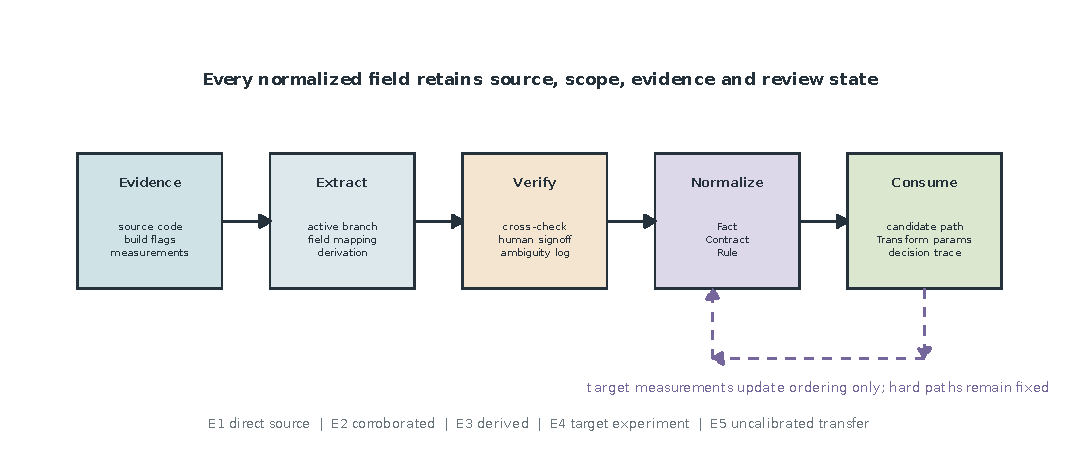
\includegraphics[width=\textwidth]{../experiments/chapter3_rules/figures/fig3-3_evidence_normalization_flow.pdf}
  \caption{专家知识的证据链、归一化与反馈流程。源码、构建和测量证据经过抽取、交叉检查、人工签核与歧义登记，形成可由 Schema 验证的 Fact、Contract 和 Rule；运行反馈只更新软先验的置信度与排序。机器检查和人工签核保持为独立状态。}
  \label{fig:chapter3-evidence-normalization}
\end{figure}

冲突按“语义与 Transform 合法性 $>$ 当前 Target Contract $>$ 同后端 E1/E2 事实 $>$ 目标实验支持规则 $>$ 跨来源软先验”的顺序处理。更高优先级规则可以抑制低层规则，但必须记录候选值、胜出来源、被抑制来源、处理动作和 \texttt{silent\_override=false}。8 个预备 shape 共生成 19 条显式冲突，主要来自实际 shape 上界与 BLIS 缓存块之间的冲突。例如，在 $64^3$ shape 上，MC=168、KC=256、NC=4080 均超过问题维度，系统将候选上界裁剪到 64，同时保留原始 E1 事实。

多来源抽取新增 4 条结构性冲突。Haswell \texttt{f32} 上，BLIS 使用 $6\times16$，OpenBLAS 使用 $8\times4$；RVV VLEN=128 上，两个来源分别使用 $16\times4$ 和 $8\times8$。这些寄存器块分别属于不同 packing 与 ABI，因此保留为后端专属硬 Contract。Haswell 的 MC/KC/NC 与 P/Q/R，以及 RVV 的两组 blocking 参数，则保留为来源标记的软先验。

同预算消融进一步验证了该处理策略的必要性。在 12 个留出 workload、5 个随机种子和预算 5 下，BLIS-only 与校准多源先验相对 naive BLIS/OpenBLAS 合并分别为 1.063 倍和 1.067 倍，95\% bootstrap 区间分别为 $[1.029,1.103]$ 与 $[1.018,1.125]$。校准多源先验相对 BLIS-only 仅为 1.003 倍，区间 $[0.986,1.021]$ 跨过 1。该结果支持“不得盲目合并来源”，但不支持“多来源必然优于可靠单来源”。

同一真实在线协议还表明，在预算 5 下，离线校准和在线校准相对随机搜索分别为 1.192 倍和 1.155 倍，区间均高于 1；在线校准相对 Optuna TPE 为 1.038 倍，区间 $[0.920,1.159]$ 跨过 1。因此，实验支持软先验在低预算下改善随机起点，不支持其显著优于成熟调优器。完整基线、公平性设置和预算 25 结果在第六章集中分析，本节只用这些证据验证硬/软知识分离与校准接口的合理性。

冻结的第三章成果包记录 5 条开放歧义，包括 alignment 字节数、完整 packed affine layout、M/N fringe 位置、Haswell 到 Comet Lake 的迁移和当时缺失的 BLIS replacement。后续实现已经通过 packing pass、direct/fringe adapter 和符号检查闭合最后一项，但原始记录仍保留其历史状态。alignment、任意 stride、更多后端和跨主机泛化仍不能由当前证据消除；K230 和第二 x86 主机在返回实测数据前也不形成性能结论。

\section{贯穿案例}

本文选择 $M=192$、$K=256$、$N=256$ 的 \texttt{f32} \texttt{linalg.matmul} 作为贯穿案例，展示

\begin{equation}
\begin{aligned}
\text{Source Line}
&\rightarrow\text{Raw Fact}
\rightarrow\text{Normalized Fact}
\rightarrow\text{Contract}\\
&\rightarrow\text{Rule}
\rightarrow\text{Candidate Domain}
\rightarrow\text{Transform Parameters}
\rightarrow\text{Observed Path}
\end{aligned}
\label{eq:chapter3-provenance-chain}
\end{equation}

的完整链条。

链条起点为 \path{config/haswell/bli_cntx_init_haswell.c:54}。该行在激活分支中把 \texttt{BLIS\_FLOAT} GEMM microkernel 注册为 \path{bli_sgemm_haswell_asm_6x16}。提取器保留原始符号并生成 \path{blis.haswell.gemm.f32.kernel_symbol}；随后从 context 恢复 MR=6、NR=16，并由 kernel setup 宏独立交叉检查。相关 Fact 共同实例化 \path{haswell_f32_gemm_6x16} Contract。

Contract 要求 AVX2/FMA、$6\times16$ 寄存器块兼容性与 A/B panel packing。缓存规则从 MC=168、KC=256、NC=4080 出发，经实际 shape 裁剪后生成候选邻域；向量规则优先选择与 8 个 \texttt{f32} lane 相容的 $T_N$。贯穿候选为

\begin{equation}
(T_M,T_N,T_K,V)=(24,32,64,1).
\label{eq:chapter3-anchor-parameters}
\end{equation}

$T_M$ 为 MR 的 4 倍，$T_N$ 为 NR 的 2 倍且可被 8 lane 整除，三个 tile 均未超过 shape，因此 Contract 预测为 direct。

为与 L{\"u}cke 等人在 Transform Dialect 性能探索实验中采用的外部调优接口对齐\cite{Luecke2025TransformDialect}，本文将其参数化 batch matmul 接口投影到普通 GEMM：

\begin{equation}
(\texttt{tile0},\texttt{tile1},\texttt{tile2},\texttt{tile3},\texttt{do\_vect})
\mapsto
(\varnothing,T_M,T_N,T_K,V)
=
(\varnothing,24,32,64,1).
\label{eq:chapter3-case45-mapping}
\end{equation}

原实验的 payload 为 $B=6$、$M=196$、$N=256$、$K=2304$ 的 \texttt{linalg.batch\_matmul}；本文 payload 不含 batch 维，因此删除 \texttt{tile0}，而不是把两个 workload 或最优配置视为相同。原实验固定的 4-lane 条件也不直接迁移，本文 lane 数由目标 Contract 推导。

\begin{figure}[!htbp]
  \centering
  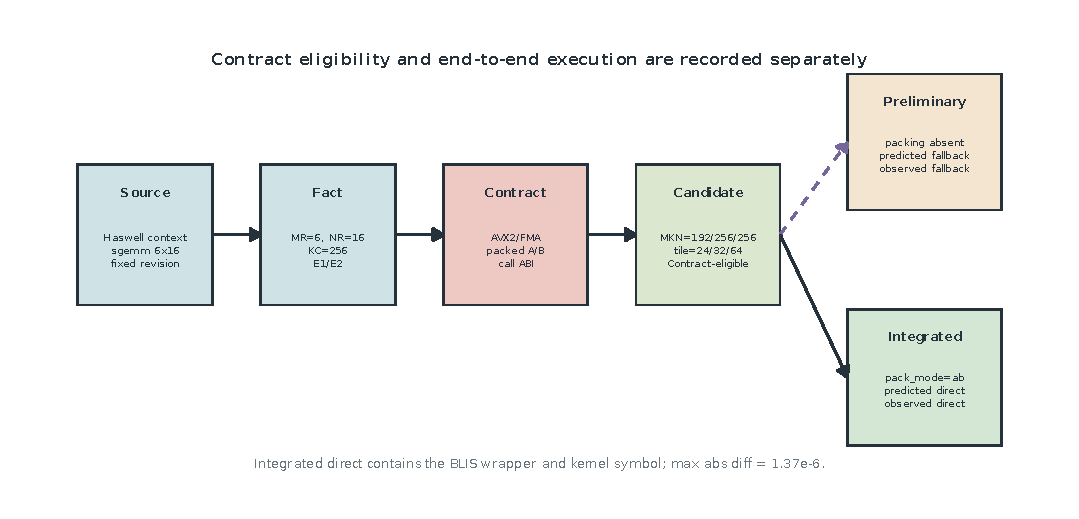
\includegraphics[width=\textwidth]{../experiments/chapter3_rules/figures/fig3-4_provenance_case.pdf}
  \caption{$192\times256\times256$ 单精度 GEMM 的端到端 provenance。相同的源码事实、Contract 和 Transform 候选在冻结预备模板中因 adapter 缺失而观测为 fallback；补齐 A/B packing 和调用适配器后，预测与观测均为 direct，生成 LLVM IR 和可执行文件包含 BLIS wrapper 与微内核符号，且两条路径均通过数值正确性检查。}
  \label{fig:chapter3-provenance-case}
\end{figure}

图~\ref{fig:chapter3-provenance-case} 保留了实现演进前后的两次观测。冻结预备实验成功应用 $(24,32,64)$ tiling 并完成编译和正确性检查，但没有 packed panel 与 BLIS 调用，故“预测 direct、观测 fallback、replacement=false”。后续集成路径使用注册 packing pass 物化 A/B panel，并由 \texttt{transform.buddy.call\_microkernel} 只负责重定向已准备好的调用占位符；LLVM IR 包含 \texttt{buddy\_blis\_sgemm\_6x16} 调用，可执行文件包含对应 BLIS kernel 符号，故“预测 direct、观测 direct、replacement=true”。同一候选在非整除 shape 上还通过 runtime fringe 计数验证了 adapt 路径。

该案例说明，provenance 不只是记录一个最终参数，而是把“知识来源、兼容性预测、实现能力和运行观测”分开保存。若适配器尚未实现，Contract 不会被回写为错误；若适配器后来补齐，也不会修改早期 raw CSV。第四章将以这一对象生成专家核心与探索外壳，第五章再说明 packing、Transform 扩展操作和调用适配器的具体实现。

\section{本章小结}

本章提出了面向 GEMM 调度空间生成的专家知识获取与统一建模方法。核心结论不是把高性能库参数直接搬入 MLIR，而是区分可迁移范围不同的两类知识：dtype、ISA、MR/NR、packing 和 call ABI 等兼容性知识必须绑定实际目标后端并形成硬 Contract；cache blocking、向量化偏好和候选排序等性能知识必须保留来源与作用范围，在目标测量前保持为软先验，并允许在线反馈校准。

在成果与证据方面，BLIS Haswell 主路径生成 22 条字段级 Fact、2 个真实微内核 Contract 和 5 类 Expert Rule，字段覆盖率、源码可追溯率和机器检查通过率均为 100\%，16 条人工核验全部签核。多来源扩展形成 4 个来源--目标 profile 和 4 条显式冲突，验证了相同 ISA 下的不同寄存器块不能脱离 packing 与 ABI 合并。单精度 1256 个实测案例和双精度 3024 条候选观测均达到 100\% 的预测--运行路径一致性；小预算实验则表明校准先验优于随机与 naive 多源合并，但未显著优于 Optuna 或可靠 BLIS-only 先验。

上述结果支持 Fact、Contract 与 Rule 三层表示以及硬/软知识分离，不支持“专家知识必然找到全局最优”或“多来源必然更强”的结论。下一章将在这些对象之上定义合法集合、执行路径、专家核心和探索外壳，并生成可由 Transform Dialect 与外部调优器执行的微内核感知搜索空间。
